\documentclass[12pt,a4paper]{article}
\usepackage[utf8]{inputenc}
\usepackage{siunitx}
\sisetup{binary-units=true,per-mode=symbol}
\usepackage[hang, flushmargin]{footmisc}
\usepackage[hyperfootnotes=false]{hyperref}
\usepackage{footnotebackref}
\usepackage{ulem,setspace}
\usepackage[labelfont=bf]{caption,subcaption}
\usepackage{graphicx,pgfplots,pgf-pie}
\usepackage{multicol}
\usepackage{minted}
\usepackage[german]{babel}
\usepackage{german}
\pgfplotsset{compat=1.9}
\normalem
\parindent 9pt
\newcommand{\rom}[1]{\uppercase\expandafter{\romannumeral #1\relax}}
\title{Institutsprojekt: Optischer Link}
\author{Raphael Brandis \and Kevin Läufer}
\date{\today}

\begin{document}
\begin{titlepage}
\begin{center}

% Upper part of the page. The '~' is needed because \\
% only works if a paragraph has started.

\includegraphics[width=0.7\textwidth]{../iph_logo.png}~\\[1cm]

\textsc{\LARGE Institut für integrierte Photonik}\\[0.5cm]

\textsc{\Large der}\\[0.5cm]

\textsc{\LARGE RWTH Aachen University}\\[1.5cm]


\textsc{\Large Institutsprojekt}\\[0.5cm]

% Title
\rule{\linewidth}{0.5mm} \\[0.4cm]
{ \huge \bfseries Optischer Link \\[0.4cm] }

\rule{\linewidth}{0.5mm} \\[1.5cm]

% Author and supervisor
\begin{minipage}[t]{0.4\textwidth}
\vspace{0pt}
\begin{flushleft} \large
\emph{Teilnehmer:}\\
Raphael \textsc{Brandis}\\
Kevin \textsc{Läufer}
\end{flushleft}
\end{minipage}
\hfill
\begin{minipage}[t]{0.4\textwidth}
\vspace{0pt}
\begin{flushright} \large
\emph{Betreuer:} \\
Johannes \textsc{Hauck}
\end{flushright}
\end{minipage}

\vfill

% Bottom of the page
{\large \today}

\end{center}
\end{titlepage}


%\maketitle
%\vfill

\tableofcontents
\newpage

\section{Aufgabenstellung}
Wir sind Studenten der Elektrotechnik an der RWTH Aachen und haben unser Viertsemester-Institutsprojekt am Institut für Integrierte Photonik (IPH) absolviert. Im Rahmen dieses Projekts haben wir uns mit der Übertragung von Informationen über optische Links beschäftigt.

Im ersten von zwei Projektteilen ging es zunächst um Informationsübermittlung mittels eines extern modulierten Laserstrahls. Anschließend sollte im zweiten Abschnitt des Projekts eine Laserdiode direkt moduliert und auf diese Weise digitale Daten übertragen werden.


\section{Extern modulierter Laser}
Um mit einem mit konstanter Intensität strahlenden Laser Informationen zu übertragen, muss mindestens ein Parameter des Laserstrahls extern moduliert werden. Mögliche Modulationsparameter sind beispielsweise die Amplitude oder die Phase des Laserstrahls. In unseren Versuchen kam ausschließlich Amplitudenmodulation zum Einsatz.

Wenn die Amplitude eines Laserstrahls extern moduliert werden soll, sind wiederum verschiedene Aufbauten als Modulator denkbar. Ein Lautsprecher mit einem in der Mitte der Membran angebrachten kleinen Spiegel kann je nach Auslenkung der Membran die Intensität des auf der Photodiode des Empfängers auftreffenden Lichts verändern; mit dieser Technik hat sich eine zweite Projektgruppe genauer beschäftigt. Wir haben uns stattdessen für die Variante entschieden, bei der ein einzelner LCD-Pixel\footnote{engl. \textit{liquid crystal display}} zum Einsatz kommt.

\subsection{LCD-Modul als Modulator}
Ein einzelner Pixel eines LCD besteht üblicherweise aus einer Flüssigkristallschicht, an die über zwei Elektroden ein elektrisches Feld angelegt werden kann, sowie einem horizontalen und einem vertikalen Polarisationsfilter, je einer vor und einer hinter der Kristallschicht.

Wären die Flüssigkristalle nicht vorhanden, würden beide Polarisationsfilter zusammen das gesamte einfallende Licht herausfiltern. Die zusätzliche Kristallschicht zwischen beiden Filtern sorgt jedoch für eine Drehung der Polarisation des durch den ersten Filter polarisierten Lichts. Da sich die Ausrichtung der Kristalle über das angelegte Feld beziehungsweise über die angelegte Spannung steuern lässt, lässt sich somit auch die Menge des insgesamt durchgelassenen Lichts steuern.

Da in unseren Versuchsaufbauten eine Laserdiode als Lichtquelle diente, war das in den Modulator einfallende Licht bereits polarisiert. Der von uns verwendete LCD-Pixel musste daher nur über einen Polarisationsfilter hinter der Kristallschicht verfügen.

\subsubsection{Übertragungscharakteristik}
\label{sec:lcd_transfer_characteristics}

Um das Übertragungsverhalten des verwendeten LCD-Modulators zu ermitteln, haben wir zunächst einen sehr einfachen Versuchsaufbau verwendet: Der Modulator wurde direkt an einen \textit{Rigol DG1022}-Signalgenerator angeschlossen, als Empfänger diente eine kommerziell erhältliche Photodiode mit integrierter Biasspannung. Mit dem Oszilloskop konnten wir nun die Amplitude des empfangenen Signals bei Übertragung von Sinusschwingungen verschiedener Frequenzen messen.

\begin{figure}[H]
  \centering
    \begin{tikzpicture}
      \begin{semilogxaxis}[
        log ticks with fixed point,
        xlabel={Frequenz [Hz]},
        ylabel={Spannung [dB]},
        xmin=9.1,
        xmax=1200,
        ymin=0,
        ymax=66,
        width=0.94\textwidth,
        height=0.57\textwidth,
        axis x line=bottom,
        axis y line=left
      ]
      \addplot+[smooth] table [x=f, y=u_db, col sep=comma] {2.1_lcd_sweep_data.csv};
      \end{semilogxaxis}
    \end{tikzpicture}
  \caption{Übertragungscharakteristik des LCD-Modulators (Trägerfrequenz: \SI{100}{\kilo\hertz}, Amplitude: $\pm$\SI{6}{\volt})}
  \label{fig:lcd_transfer_function}
\end{figure}

In unseren Messungen fiel die Amplitude schon im niedrigen zweistelligen Frequenzbereich stark ab. Bei einer von \SI{10}{\hertz} ausgehenden Messreihe war der \SI{-3}{\decibel}-Punkt bereits bei cirka \SI{20}{\hertz} erreicht. Durch Verwendung einer hochfrequenten Trägerwelle, die mit dem niederfrequenten Nutzsignal amplitudenmoduliert wurde\footnote{Diese Funktion stellte der verwendete Signalgenerator von Haus aus bereit.}, ließ sich das Übertragungsverhalten geringfügig verbessern (siehe Abbildung \ref{fig:amplitude_modulation}). Insgesamt mussten wir dennoch feststellen, dass sich der von uns verwendete LCD-Pixel aufgrund seiner geringen Geschwindigkeit nur eingeschränkt als Modulator zur Informationsübertragung eignet (siehe Frequenzgang in Abbildung \ref{fig:lcd_transfer_function}).

\begin{figure}[H]
  \centering
    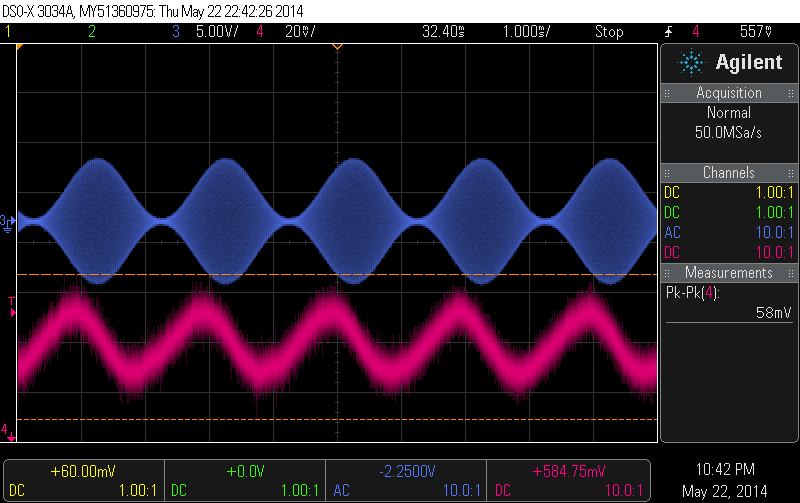
\includegraphics[width=0.8\textwidth]{../measurements/20140522_sweep/scope_1.png}
  \caption{Blau: AM-modulierte Trägerwelle, Rosa: Empfangenes Signal}
  \label{fig:amplitude_modulation}
\end{figure}


\subsection{Übertragung von Audiosignalen}

Im nächsten Schritt sollten statt einfachen Sinussignalen, die sich direkt im Signalgenerator erzeugen lassen, komplexere Audiosignale mithilfe unseres analogen Links übertragen werden --- beispielsweise Musik.

Aufgrund der in Abschnitt \ref{sec:lcd_transfer_characteristics} erläuterten Versuchsergebnisse war es unser Ziel, den Modulator weiterhin mit einer hochfrequenten, amplitudenmodulierten Trägerwelle anzusteuern. Da der Modulationseingang des Signalgenerators nach einem Pegel von $\pm$\SI{5}{\volt} verlangte, haben wir zunächst auf dem Breadboard eine diskrete Kopfhörerverstärkerschaltung aufgebaut, die das aus einem Smartphone oder einem Computer kommende Musiksignal auf den nötigen Pegel verstärkt.

Auf der Empfängerseite kam eine ebenfalls diskret aufgebaute Transimpedanzverstärkerschaltung zum Einsatz, an die zwei aktive Lautsprecher angeschlossen wurden. Der Aufbau aus Laserdiode, LCD-Modulator und Photodiode mit Transimpedanzverstärker ist in Abbildung \ref{fig:photo_lcd_experiment} zu sehen.

\begin{figure}[H]
  \centering
    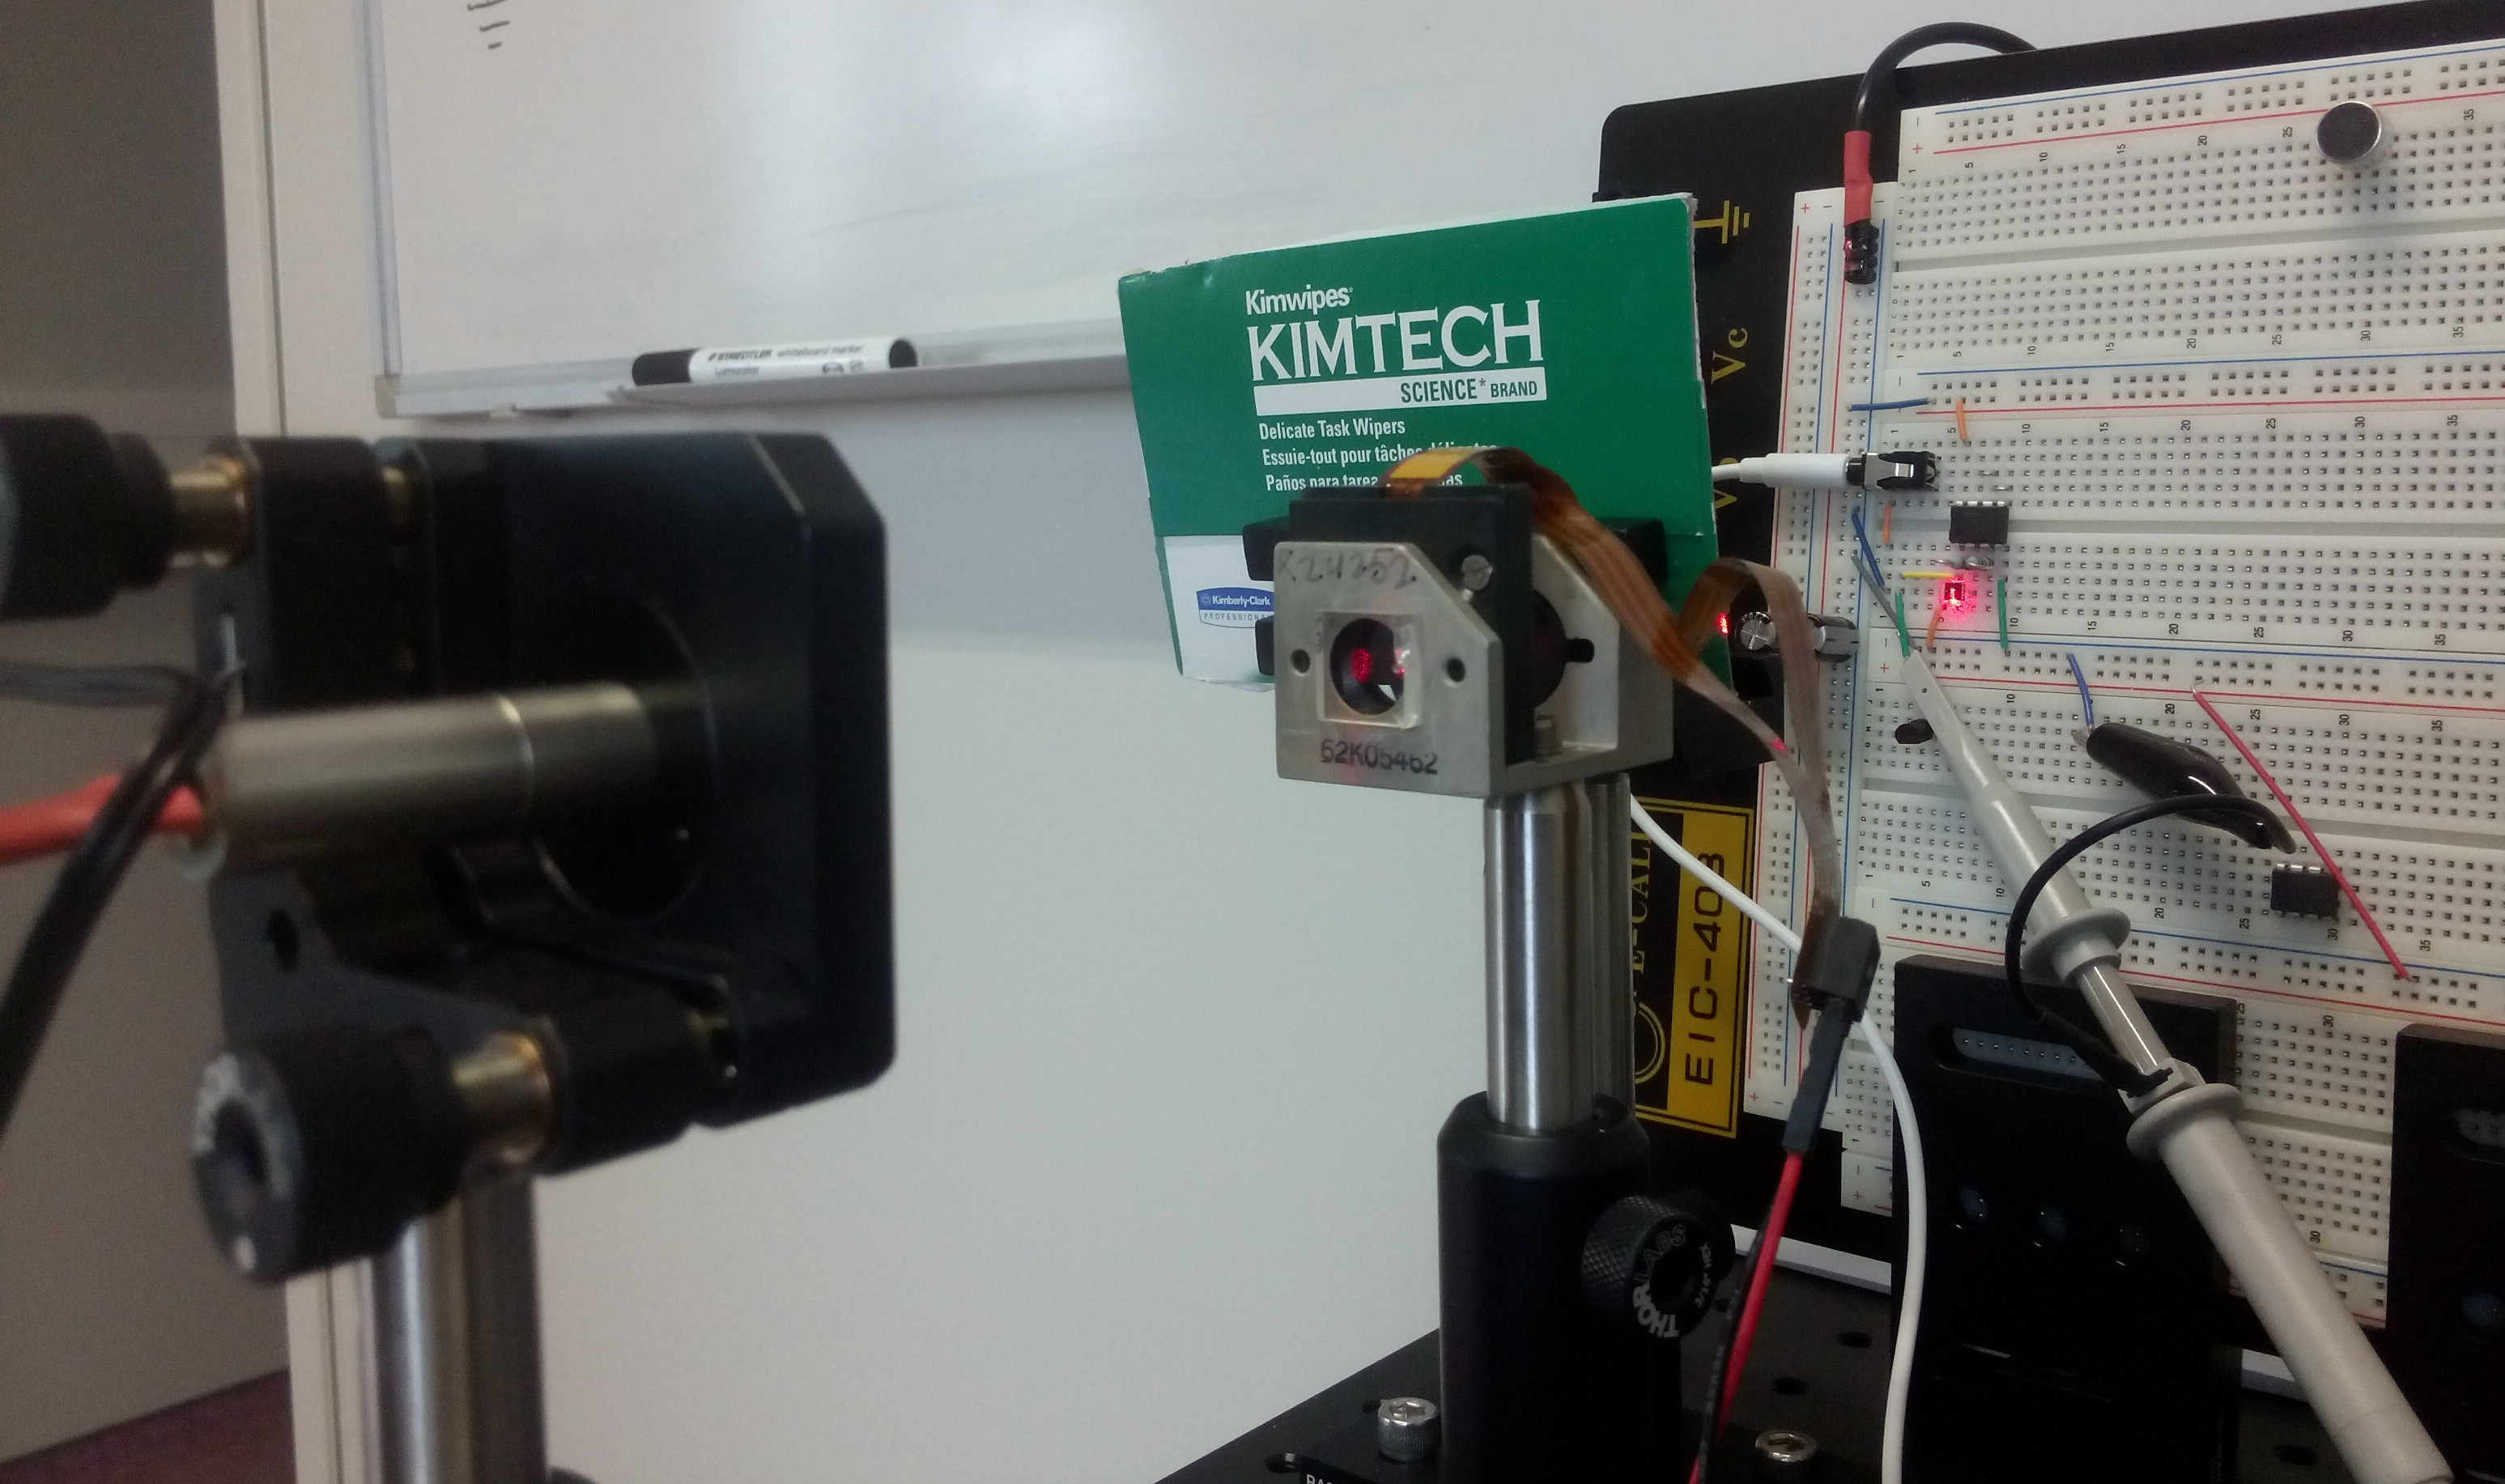
\includegraphics[width=\textwidth]{img/photo_lcd_experiment.jpg}
  \caption{Versuchsaufbau zur Übertragung von Audiosignalen}
  \label{fig:photo_lcd_experiment}
\end{figure}

War bei der Übertragung einzelner Sinustöne der Ton noch bis in hohe Frequenzbereiche ($>$\SI{10}{\kilo\hertz}) hörbar, so verschlechterte sich das Übertragungsverhalten für breitbandige Musiksignale sehr stark. Erst durch eine Bandbreitenbegrenzung der Musik auf Frequenzen bis maximal \SI{750}{\hertz} wurden einzelne Basstöne aus dem Ursprungssignal erkennbar, die jedoch weiterhin von starken Störgeräuschen und Verzerrungen begleitet wurden.

\begin{figure}[H]
  \centering
  \begin{subfigure}[b]{1.0\textwidth}
    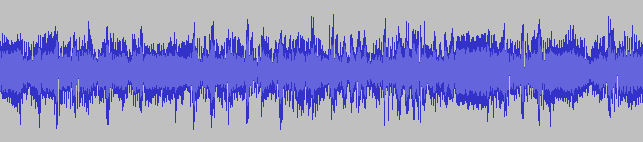
\includegraphics[width=\textwidth]{../audacity_sent.png}
    \caption{Bandbreitenbegrenztes Ursprungssignal}
    \label{fig:audacity_sent}
  \end{subfigure}  
  \begin{subfigure}[b]{1.0\textwidth}
    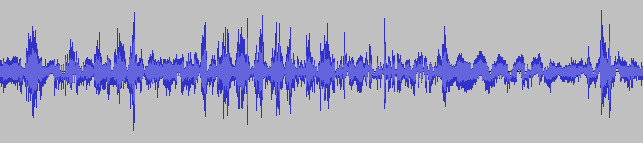
\includegraphics[width=\textwidth]{../audacity_received.png}
    \caption{Mit einem Mikrofon aufgezeichnete Ausgabe der Lautsprecher}
    \label{fig:audacity_received}
  \end{subfigure}  
  \caption{Übertragung eines Musiksignals}
  \label{fig:audacity}
\end{figure}

In Abbildung \ref{fig:audacity} ist die geringe Übereinstimmung der Wellenformen des zu übertragenden Musiksignals (\ref{fig:audacity_sent}) und des aus den Lautsprechern zu hörenden Signals (\ref{fig:audacity_received}) zu erkennen.

Auch bei reinen Sprachsignalen reichte die Übertragungsqualität bei weitem nicht aus, um Sprachverständlichkeit zu gewährleisten.

\subsection{Übertragung digitaler Daten}
Nach den Experimenten mit der analogen Signalübertragung war es von Interesse, auch einmal digitale Daten über den bestehenden optischen Link zu übertragen.

\subsubsection{USB-UART-Dongle}
In einem ersten Ansatz wurden günstige UART\footnote{Universal Asynchronous Receiver / Transmitter}-USB-Adapter verwendet. Die Adapter arbeiten mit \SI{3.3}{\volt}-CMOS-Signalen, die mittels eines Komparators auf den nötigen Pegel von $\pm$\SI{5}{\volt} gebracht werden. Mit diesem Pegel lässt sich der Eingang des \textit{Rigol DG1022}-Signalgenerators ansteuern. Bei Amplitudenmodulation führen dann +\SI{5}{\volt} zur maximalen Amplitude und -\SI{5}{\volt} zu einer Amplitude von fast Null. So ließ sich ein einfaches On-Off-Keying umsetzen.

Leider war es nicht möglich, bei den verwendeten UART-Adaptern Baudraten unter \SI{1}{\kilo\hertz} einzustellen. Dies war aber deutlich zu schnell für das LCD, wie man in Abbildung~\ref{fig:uart_continous_key} sehen kann. Hier wurde am Computer eine Taste im Terminal gedrückt gehalten, um immer den gleichen Wert zu senden.

Man beachte, dass bei dieser und allen folgenden Messungen der grüne Kanal, also die Messung am Ausgang des Transimpedanzverstärkers, auf AC Coupling eingestellt war. Somit sind die Messergebnisse nicht verlässlich und es lassen sich höchstens Tendenzen feststellen. Hier wäre es interessant, die Messungen noch einmal mit richtigen Einstellungen zu wiederholen.

Dennoch ist klar erkennbar, dass ein kurzes \textit{High} am Ausgang des UART-Adapters (blauer Kanal) zu wenig Änderung am Ausgang des Transimpedanzverstärkers führt. Das LCD kann dem Signal vermutlich nicht schnell genug folgen.


\begin{figure}[H]
  \centering
    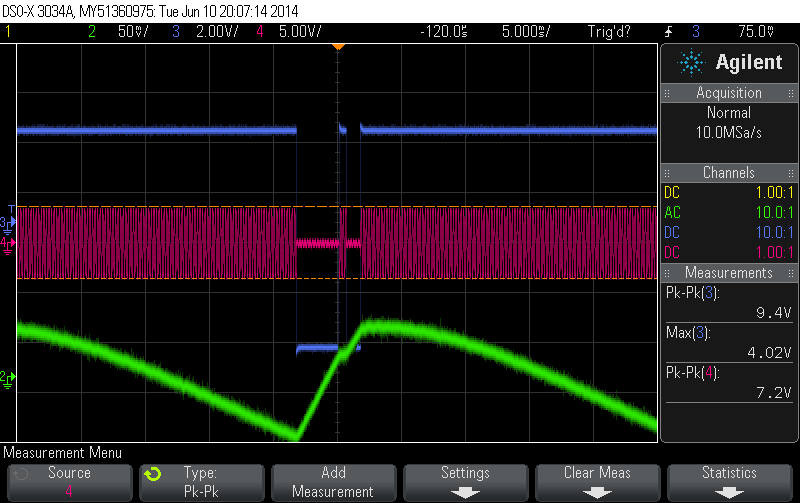
\includegraphics[width=0.8\textwidth]{../measurements/20140610/uart_continous_key/scope_0.png}
  \caption{Hier wird kontinuierlich der gleiche Wert mittels UART gesendet.}
  \label{fig:uart_continous_key}
\end{figure}

\subsubsection{Datenübertragung mit 10 Hz}
Nachdem die UART-Adapter nicht langsam genug Daten liefern konnten, wurde als nächstes ein weiterer Signalgenerator verwendet, der in der Lage war, Bitsequenzen mit einer bestimmten Frequenz zu erzeugen, in unserem Fall mit \SI{10}{\hertz}. Diese Bitsequenzen wurden genutzt, um mittels On-Off-Keying das LCD anzusteuern.

Interessant ist hierbei der Unterschied zwischen einem determinierten Muster aus sich abwechselnden Nullen und Einsen und einem Zufallsmuster. Wie in Abbildung~\ref{fig:uart_10hz} gut zu sehen ist, kann sich das LCD auf eine konstante Frequenz einschwingen. Bei einem Zufallssignal hingegen hängt das Signal von der Vorgeschichte ab. Hier wird deutlich, warum bei Messungen der Signalqualität (z.B. bei der Erstellung von Augendiagrammen, siehe \ref{sec:eye_diag}) ein Zufallssignal verwendet werden sollte und ein deterministisches Signal nicht ausreicht.

\begin{figure}[H]
  \centering
  \begin{subfigure}[b]{0.7\textwidth}
    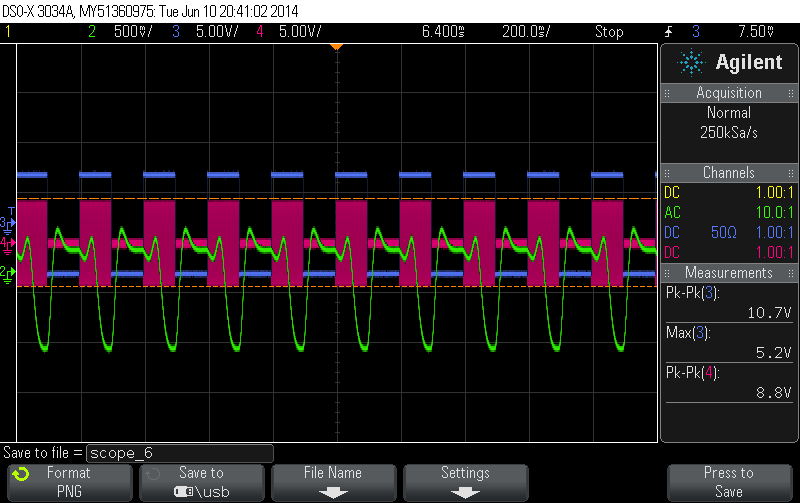
\includegraphics[width=\textwidth]{../measurements/20140610/10Hz_toggle/scope_6.png}
    \caption{Abwechselnde Nullen und Einsen}
    \label{fig:uart_10hz_toggle}
  \end{subfigure}
  \begin{subfigure}[b]{0.7\textwidth}
    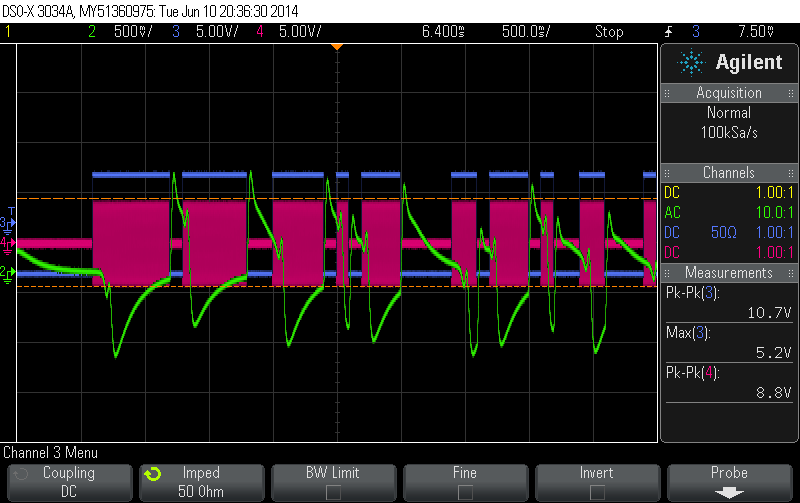
\includegraphics[width=\textwidth]{../measurements/20140610/10Hz_random/scope_4.png}
    \caption{Zufälliges Signal}
    \label{fig:uart_10hz_random}
  \end{subfigure}
  \caption{Übertragung verschiedener \SI{10}{\hertz}-Signale}
  \label{fig:uart_10hz}
\end{figure}

\subsubsection{Software-UART mit Mikrocontrollern}
Um nun endlich digitale Nutzdaten zu übertragen, haben wir auf einem Mikrocontroller UART in Software implementiert, um die verwendete Baudrate beliebig niedrig wählen zu können. Hierzu wurden zwei \textit{STMicroelectronics Discovery Boards} verwendet, eines mit \textit{STM32F4}- und eines mit \textit{STM32F3}-Mikrocontroller. Der Quellcode nutzt die \textit{XPCC}-Bibliothek und ist auf \url{http://github.com/ekiwi/iph} abrufbar. Die wichtigsten funktionalen Bestandteile sind aber auch im Anhang~\ref{app:code} zu finden.

Zur Verbesserung der Robustheit der Übertragung kam ein (7,4)-Hamming-Code zum Einsatz, bei dem alle gültigen Codewörter untereinander einen Hammingabstand von mindestens drei besitzen. Somit kommen auf vier Datenbits drei Paritätsbits, was die Korrektur einfacher Bitfehler erlaubt. Ein möglicher Algorithmus hierfür sieht wie folgt aus (siehe auch Quellcode in Anhang~\ref{app:code_hamming}):

Für ein empfangenes Wort wird der Hammingabstand zu jedem gültigen Codewort errechnet. Beträgt der Abstand eins oder null, wird davon ausgegangen, dass das empfangene Wort dem Codewort entspricht. Bei zweifachen Bitfehlern führt dies zu einer falschen Zuordnung: Da der Hammingabstand zwischen zwei gültigen Codeworten drei beträgt und bei zwei Bitfehlern der Abstand zum ursprünglichen Codewort zwei ist, gibt es ein anderes Codewort, zu dem die empfangene Sequenz nur einen Hammingabstand von eins hat. Diesem Codewort wird das empfangene Wort fälschlicherweise zugeordnet.

\begin{figure}[H]
  \centering
  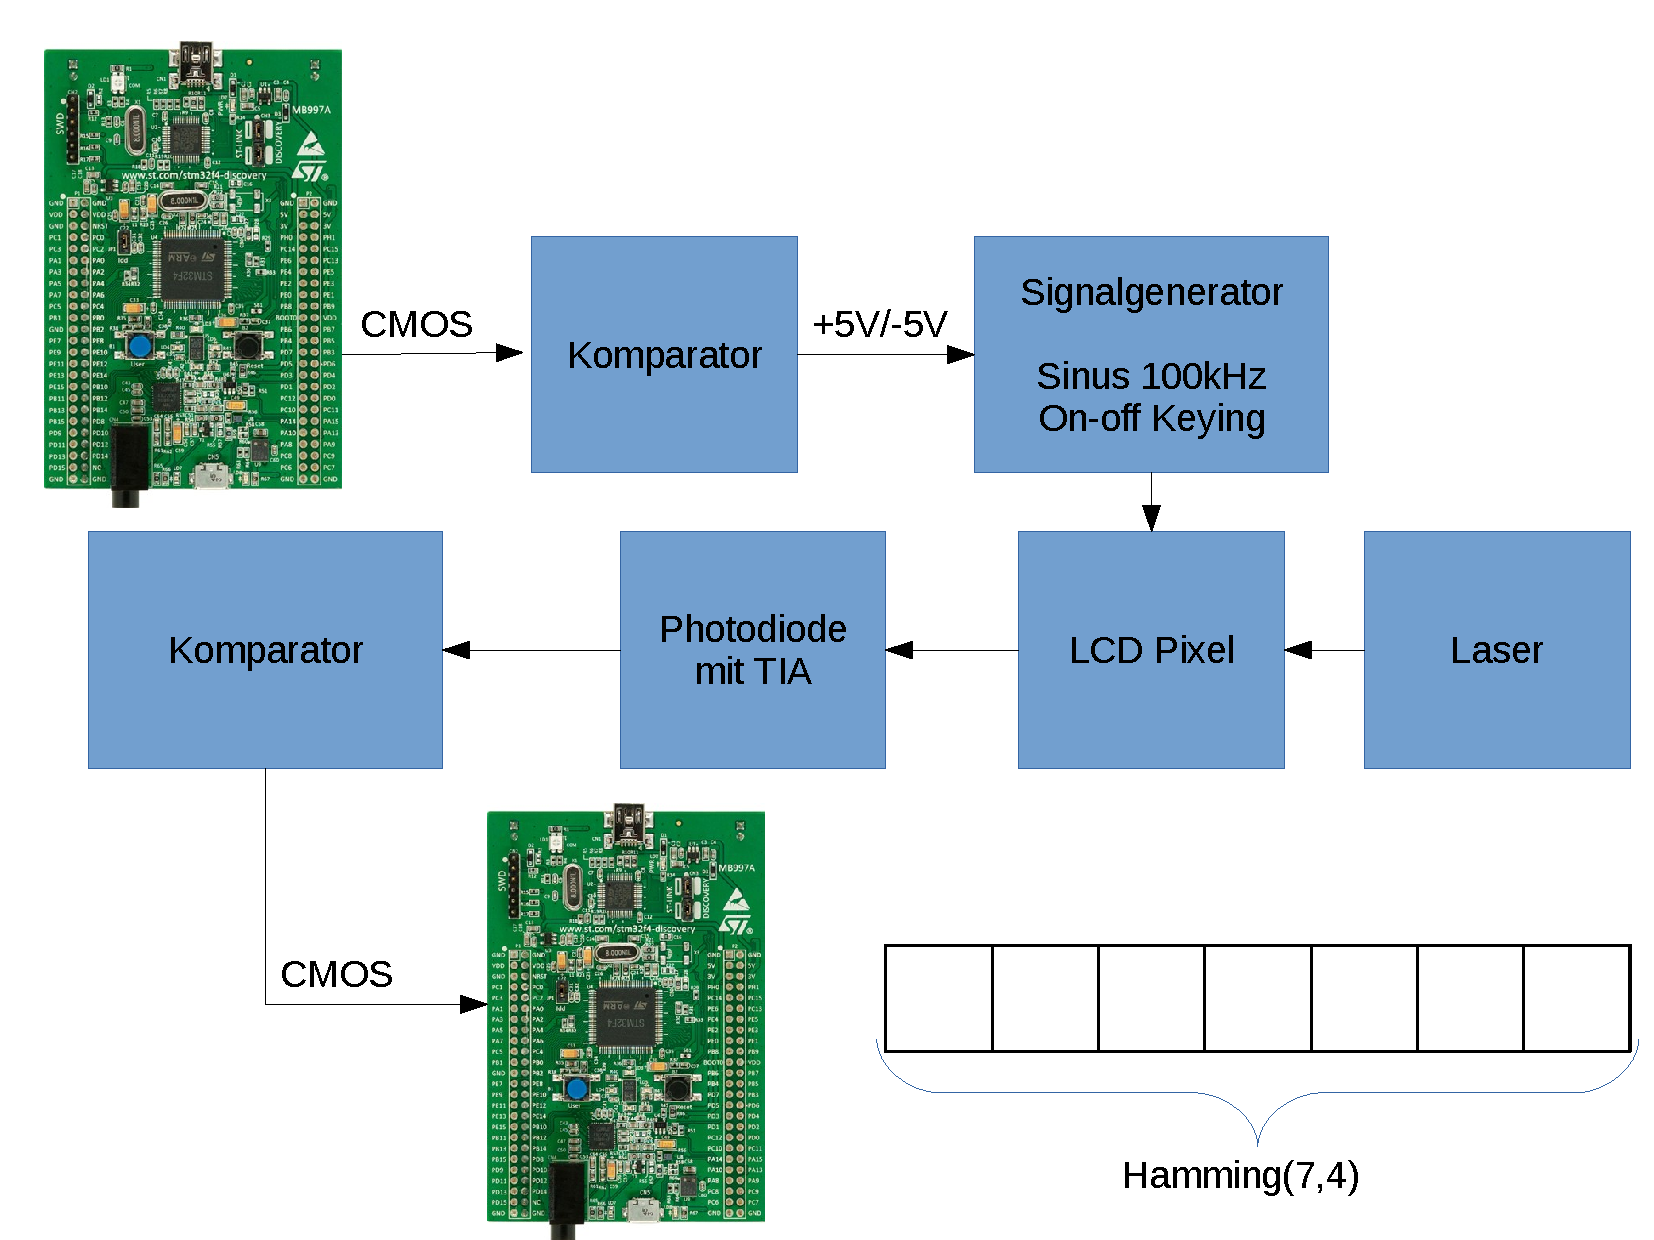
\includegraphics[width=\textwidth]{img/software_uart.pdf}
  \caption{Software-UART-Signalkette}
  \label{fig:sotware_uart_signal_chain}
\end{figure}


Zum Test der Übertragung wurden 294 Datenwörter in (7,4)-Hamming-Codierung übertragen. Der Versuchsaufbau ist in Abbildung~\ref{fig:sotware_uart_signal_chain} dargestellt. Die Positionierung des Lasers und der Empfängerdiode entsprachen dem in Abbildung~\ref{fig:photo_lcd_experiment} gezeigten Aufbau. Der Inhalt der Datenpakete waren die Zahlen von 0 bis 15. Dies reduziert die Aussagekraft des Experiments etwas im Vergleich zu randomisierten Daten, erleichterte aber die Auswertung erheblich. Um nämlich zwei oder mehr Bitfehler erkennen zu können, müssen die gesendeten Daten am Empfänger bekannt sein. Somit gelangten wir zu der in Abbildung~\ref{fig:sotware_uart_errors} dargestellten Fehlerverteilung.

\begin{figure}[H]
  \centering
    \begin{tikzpicture}
    \pie[explode=0.1,color={green,yellow,orange}]{26/0 Fehler, 62/1 Fehler, 12/2+ Fehler}
    \end{tikzpicture}
  \caption{Fehler bei der Übertragung von 294 (7,4)-Hamming-codierten, deterministischen Datenworten mit einem \SI{4}{\hertz}-UART-Signal}
  \label{fig:sotware_uart_errors}
\end{figure}

Demnach sind, nach Fehlerkorrektur durch den Hammingcode, immer noch \SI{12}{\percent} der empfangenen Daten falsch und müssten in einem echten Übertragungssystem durch höhere Layer abgefangen werden. Die Rate der Datenbits berechnet sich wie folgt:

\begin{equation}
 \SI{4}{\bit\per\second} * \frac{\SI{4}{\bit}}{\SI{7}{\bit}} \approx \SI{2.3}{\bit\per\second}
\end{equation}

Somit wurden über etwa \SI{30}{\centi\meter} mit \SI{2.3}{\bit\per\second} und einer recht hohen Fehlerrate von \SI{12}{\percent} Daten übertragen --- kein sehr gutes Ergebnis.

Doch wie ist dieses schlechte Resultat zu erklären? Für eine Erklärungsversuch lohnt es sich, die Messungen in Abbildung~\ref{fig:uart_4hz_edge} zu betrachten. Hier sieht man, dass eine zufällig ausgewählte steigende Flanke (\ref{fig:uart_4hz_rising_edge}) \SI{162}{\milli\second} benötigt, um durch das System zu propagieren. Eine fallende Flanke (\ref{fig:uart_4hz_falling_edge}) hat mit \SI{20}{\milli\second} eine deutlich kleinere Verzögerung. Weitere beobachtete Flanken wiesen Verzögerungen in der gleichen Größenordnung auf.

\begin{figure}[H]
  \centering
  \begin{subfigure}[b]{0.6\textwidth}
    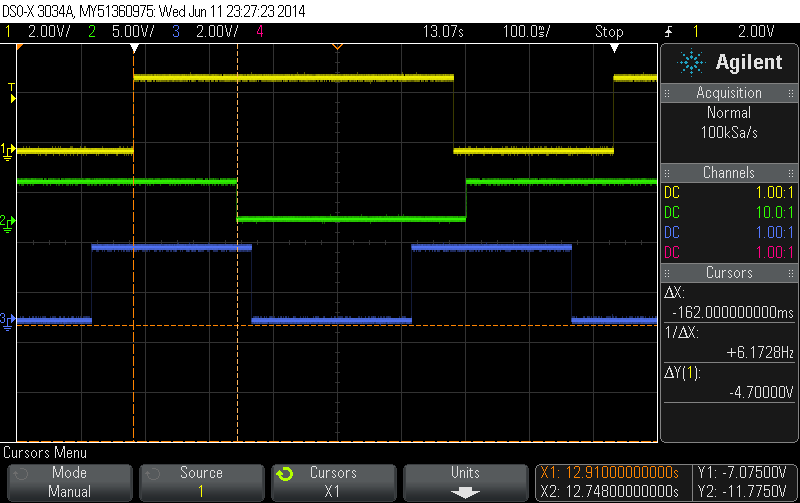
\includegraphics[width=\textwidth]{../measurements/20140611/4Hz_rising_edge/scope_2.png}
    \caption{steigende Flanke: \SI{162}{\milli\second}}
    \label{fig:uart_4hz_rising_edge}
  \end{subfigure}
  \begin{subfigure}[b]{0.6\textwidth}
    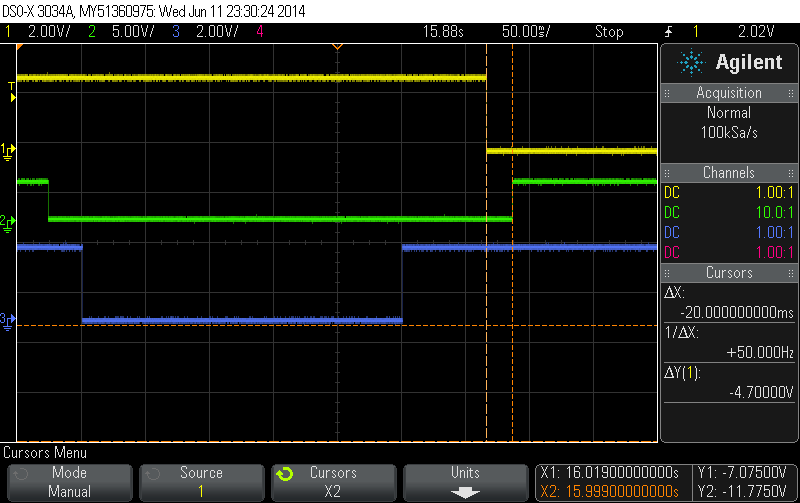
\includegraphics[width=\textwidth]{../measurements/20140611/4Hz_falling_edge/scope_6.png}
    \caption{fallende Flanke: \SI{20}{\milli\second}}
    \label{fig:uart_4hz_falling_edge}
  \end{subfigure}
  \caption{Verzögerung bei einem \SI{4}{\hertz}-UART-Signal; Quellensignal in gelb und invertiertes Ausgangssignal in grün}
  \label{fig:uart_4hz_edge}
\end{figure}

Da bei einem zufälligen Bit eine steigende Flanke sowohl an dessen Anfang als auch an dessen Ende auftreten kann, müsste man demnach mehr als \SI{162}{\milli\second} nach Anfang und \SI{162}{\milli\second} vor Ende eines Bits sampeln, um Fehler ganz zu vermeiden. Dies führt zu folgender maximaler Datenrate:

\begin{equation}
	T_{min} = \SI{162}{\milli\second} * 2 = \SI{324}{\milli\second}
\end{equation}
\begin{equation}
	f_{max} = \frac{1}{T_{min}} = \frac{1}{\SI{324}{\milli\second}} \approx \SI{3}{\bit\per\second}
\end{equation}

Ein Absenken der Bitrate auf \SI{3}{\bit\per\second} in Kombination mit einer intelligenten Wahl des Samplingzeitpunktes könnte also eine Hamming-Codierung überflüssig machen und somit zu einer höheren Datenrate führen. Hierfür müssen aber die Latenzen bekannt sein und bei der Synchronisation durch die erste fallende Flanke (siehe Anhang~\ref{app:uart_receiver}, Zeile 39) berücksichtigt werden.

Als wir bei einem Test ohne Kenntnis der Latenz mit einer Datenrate von \SI{2}{\bit\per\second} Daten übertragen haben, traten fast keine Bitfehler auf.

Die mit den oben aufgeführten Berechnungen ermittelte maximale theoretische Datenrate von etwa \SI{3}{\bit\per\second} ist jedoch weiterhin sehr niedrig. Interessant wäre es daher, die Ursache der Latenz zu untersuchen. Hierbei sollte bei verschiedenen Ansteuerungsarten des LCD die erzielte Latenz gemessen werden. Mit den oben genannten Berechnungen lässt sich daraus die mögliche Datenrate berechnen.

\section{Direkt modulierter Laser}
Im zweiten Teil des Projekts sollte ein Diodenlaser direkt moduliert werden, um damit digitale Daten zu übertragen. Dazu hatte die andere Gruppe bereits eine Modulationsmethode untersucht, bei der auf einen konstanten Strom ein Datensignal aufgekoppelt wurde.

Unser Ziel war es, eine Stromquelle direkt mit einem Datensignal zu modulieren und danach Empfängerdesigns zu evaluieren.


\subsection{Sender: Modulierte Konstantstromquelle}
\label{sec:direct_tx}

Aufgrund der exponentiellen Kennlinie einer Laserdiode muss diese mit einem konstanten Strom versorgt werden. Eine einfache Konstantstromquelle lässt sich mit zwei Bipolartransistoren aufbauen, wie in Abbildung~\ref{fig:modulated_current_source} zu sehen ist.

\begin{figure}[H]
  \centering
    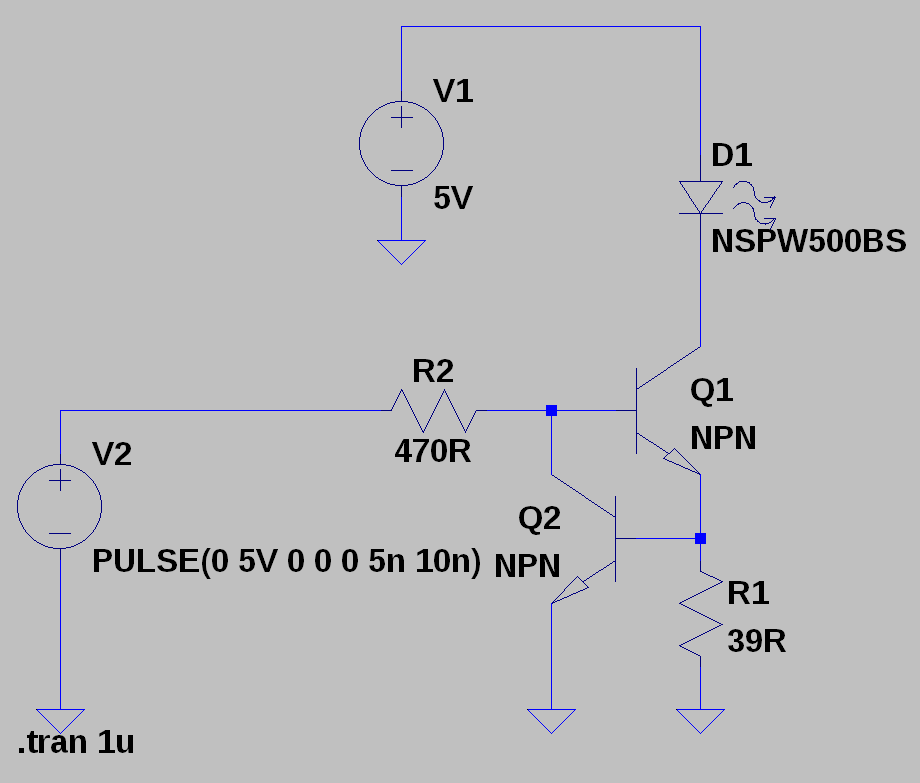
\includegraphics[width=0.8\textwidth]{../spice/modulated_current_source.png}
  \caption{Modulierte Stromquelle.}
  \label{fig:modulated_current_source}
\end{figure}

Der Strom $I_{D1}$, der durch die Diode fließt, entspricht hierbei in etwa dem Strom $I_{R1}$, der durch den Widerstand $R1$ fließt. An diesem müssen, durch den Transistor $Q2$ vorgegeben, etwa \SI{0.7}{\volt} abfallen, wodurch sich folgender Strom einstellt:

\begin{equation}
I_{D1} = I_{R1} = \frac{U_{R1}}{R1} \approx \frac{\SI{0.7}{\volt}}{R1}
\end{equation}

Diese Konstantstromquelle lässt sich leicht ein- und ausschalten, indem über einen Widerstand die Summe der Basis-Emitter-Spannungen beider Transistoren, $U_{BE1} + U_{BE2}$, vorgegeben wird.

\begin{figure}[H]
  \centering
    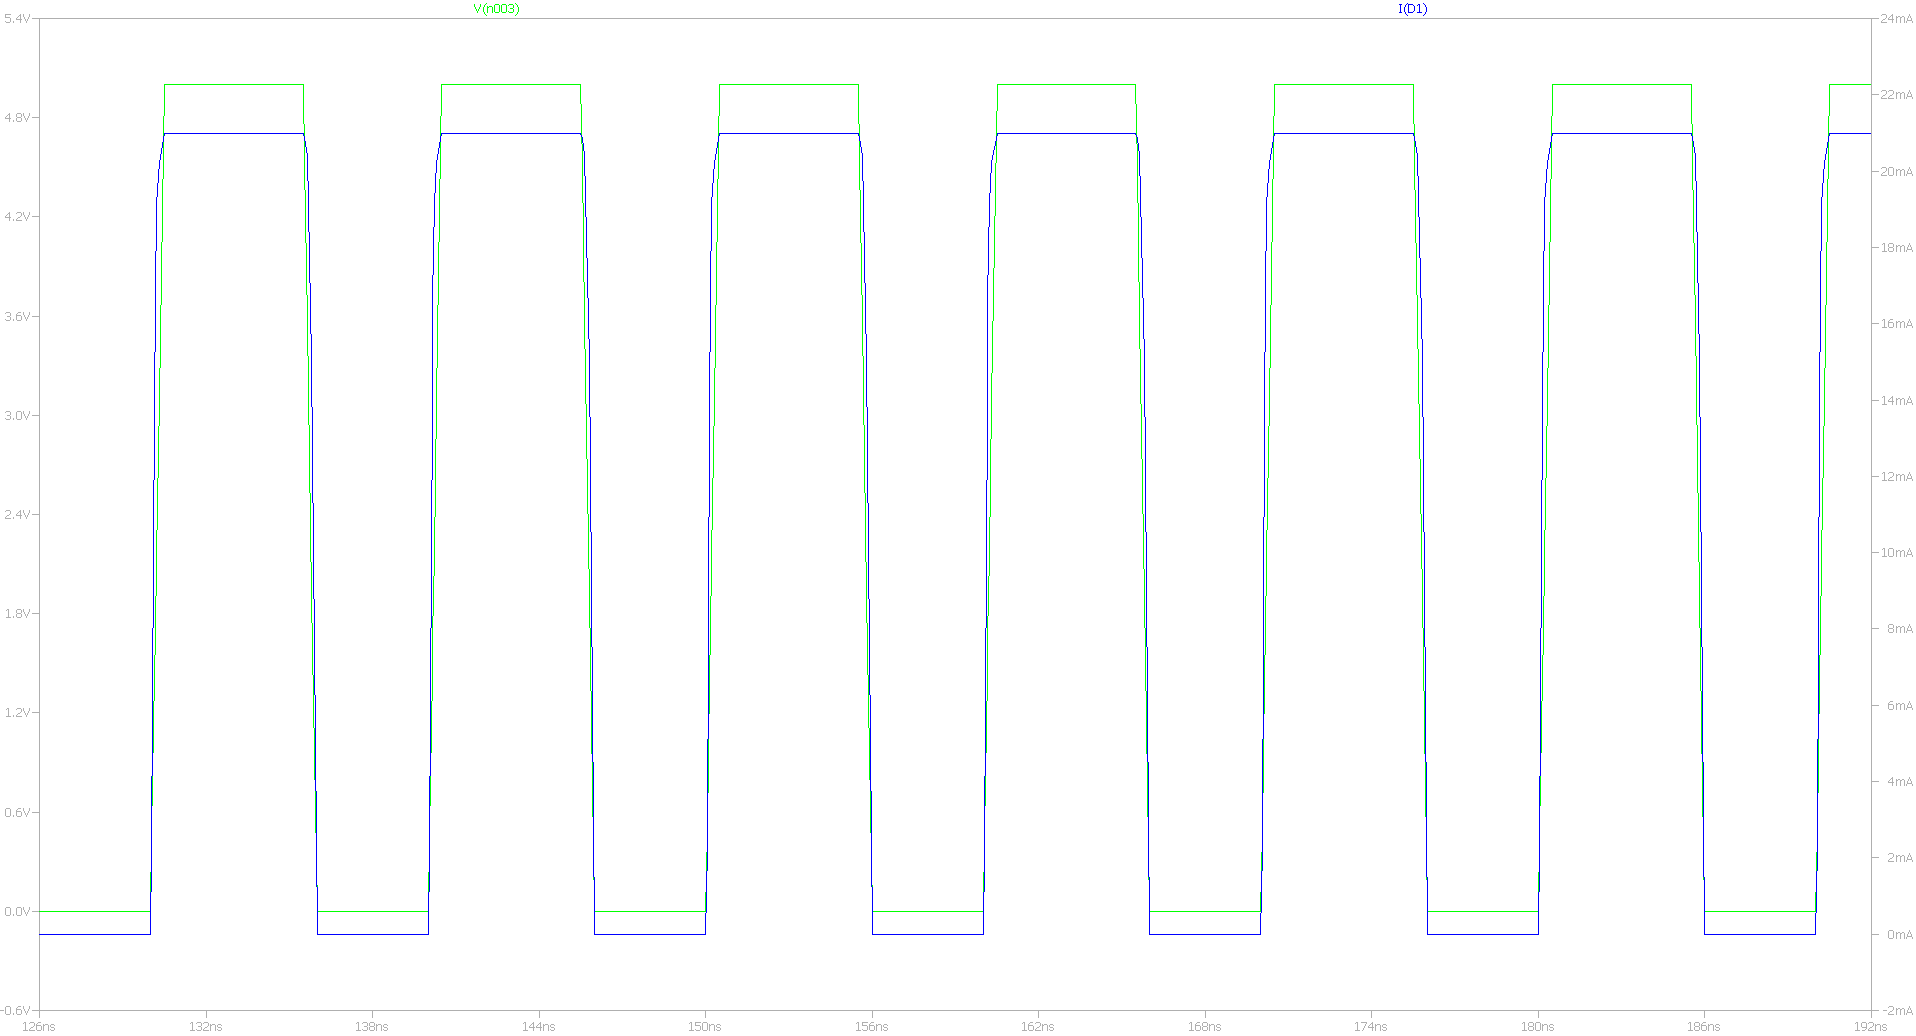
\includegraphics[width=1.0\textwidth]{../spice/current_input_v_current_out_trans.png}
  \caption{Transientenanalyse der modulierten Stromquelle}
  \label{fig:modulated_current_source_plot}
\end{figure}


Eine Simulation des Aufbaus in LTSpice zeigt, dass der Strom $I_{D1}$ durch die Diode von der Eingangsspannung $U_2$ abhängt. Bei den in Abbildung~\ref{fig:modulated_current_source_plot} dargestellten Ergebnissen wurde zwar mit einem vereinfachten Transistormodell simuliert, sie sind also mit Vorsicht zu genießen. Das Funktionsprinzip wird durch die Simulation dennoch gut veranschaulicht.

\begin{figure}[H]
  \centering
    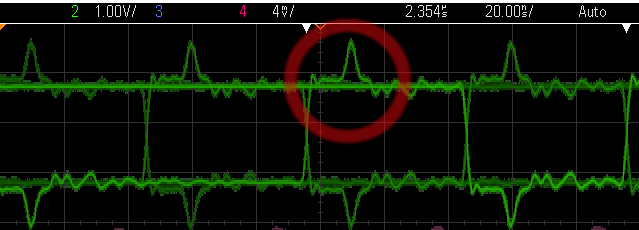
\includegraphics[width=1.0\textwidth]{img/ring_20MHz.png}
  \caption{Reflexionen bei einem \SI{20}{\mega\hertz}-Eingangssignal}
  \label{fig:ring_20mhz}
\end{figure}

Mit diesem Aufbau ließen sich in unseren Versuchen recht schnelle Übertragungen von zufälligen Bits realisieren (siehe auch Abschnitt~\ref{sec:direct_rx}). Es gab jedoch aufgrund der fehlenden Terminierung auf der Eingangsseite unserer Schaltung Probleme mit Reflexionen auf der Leitung (siehe Abbildung~\ref{fig:ring_20mhz}). Hier wäre eine Untersuchung verschiedener Terminierungsvarianten interessant.

Auch verhält sich die Schaltung bei Frequenzen im Megahertzbereich immer weniger wie in der Simulation: So entspricht die Spannung am Widerstand $R1$ nicht mehr den erwarteten \SI{0.7}{\volt}. Hier wären eine Verbesserung der Spice-Simulation durch die Auswahl eines passenden Transistormodells und durch bessere Modellierung der Quelle sowie weitere empirische Versuche angebracht.

\subsection{Photodiode mit Lastwiderstand als Empfänger}
\label{sec:direct_rx}

\begin{figure}[H]
  \centering
  \begin{subfigure}[b]{0.6\textwidth}
    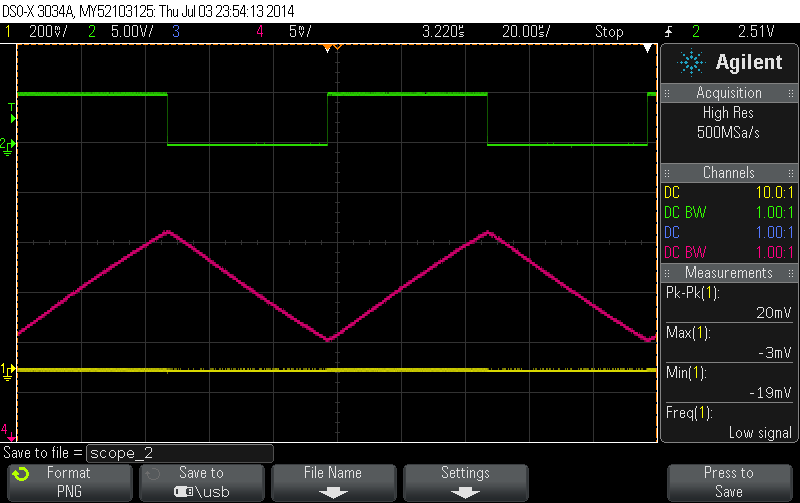
\includegraphics[width=\textwidth]{../measurements/20140703/20kHz_10kOhm/scope_2.png}
    \caption{\SI{10}{\kilo\ohm}}
    \label{fig:direct_rx_10k_R}
  \end{subfigure}  
  \begin{subfigure}[b]{0.6\textwidth}
    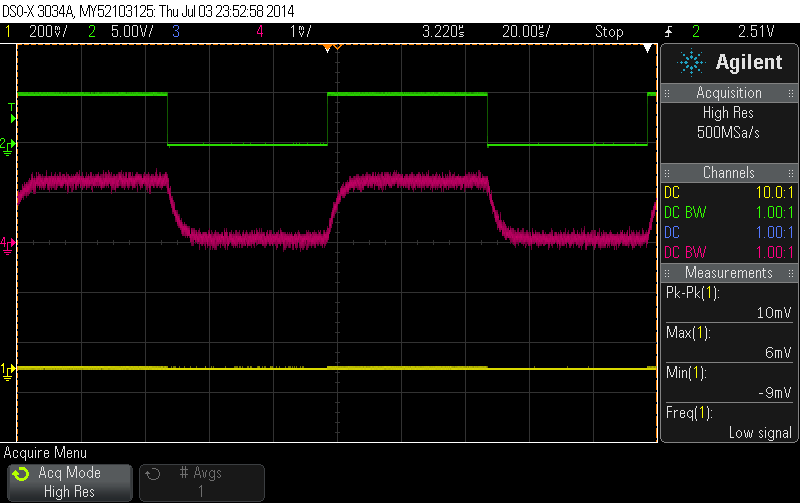
\includegraphics[width=\textwidth]{../measurements/20140703/20kHz_50_Ohm/scope_0.png}
    \caption{\SI{50}{\ohm}}
    \label{fig:direct_rx_50_R}
  \end{subfigure}  
  \caption{Grün: Gesendetes \SI{20}{\kilo\hertz}-Rechtecksignal; Rosa: Empfangenes Signal bei unterschiedlichem Lastwiderstand}
  \label{fig:direct_rx}
\end{figure}

Zum Testen der Sendeschaltung nutzten wir zunächst eine Photodiode mit Biasspannung und umschaltbarem Lastwiderstand (\textit{NewFocus 1623}) als Empfänger.

In Abbildung~\ref{fig:direct_rx} ist die Abhängigkeit des Ausgangssignals vom Lastwiderstand zu erkennen. Zur Aufnahme dieser Messungen wurde der Ausgang der Photodiode mit einem hochohmig terminierten Eingang eines Oszilloskops verbunden und auf den Eingang unserer Sendeschaltung ein \SI{20}{\kilo\hertz}-Rechtecksignal gegeben. Bei einem hohen Lastwiderstand (\ref{fig:direct_rx_10k_R}) erhöht sich die Verstärkung: Die Amplitude beträgt hier in etwa \SI{10}{\milli\volt}. Jedoch sinkt die Bandbreite, was sich durch sehr lange Anstiegs- und Abfallzeiten und die daraus resultierende Dreiecksform des Ausgangssignals bemerkbar macht. Mit einem kleineren Lastwiderstand (\ref{fig:direct_rx_50_R}) ergibt sich ein weniger verzerrtes Signal, die Amplitude beträgt jedoch nur noch in etwa \SI{1}{\milli\volt}.

Die kleinen Amplituden und die Verzerrung beim Empfang eines \SI{20}{\kilo\hertz}-Signals weisen darauf hin, dass für schnellere Signale ein besserer Verstärker benötigt wird.

\subsection{Empfänger mit integriertem \textit{AD8015} Transimpedanzverstärker}
\label{sec:direct_rx_tia}

\begin{figure}[H]
  \centering
    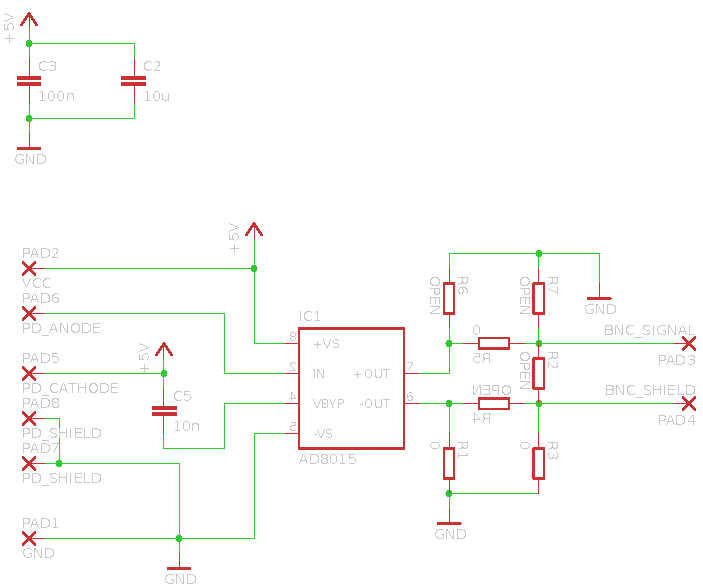
\includegraphics[width=0.7\textwidth]{img/receiver.pdf}
  \caption{Beschaltung des \textit{AD8015}-Transimpedanzverstärkers}
  \label{fig:receiver_sch}
\end{figure}

Anstatt selbst eine Empfängerschaltung aufzubauen, bietet es sich an, einen integrierten Transimpedanzverstärker wie den \textit{AD8015} zu verwenden. Dieser ist von Grund auf dafür konzipiert, den Photostrom in eine proportional verstärkte Spannung zu wandeln, die differentiell mit einer Impedanz von \SI{50}{\ohm} am Ausgang abgegriffen werden kann. Es werden nur wenige externe Komponenten benötigt, was zu einer einfachen Schaltung führt (siehe Abbildung \ref{fig:receiver_sch}).

Mit diesem Aufbau lassen sich auch schnelle Signale verstärken, wie in der Betrachtung der Augendiagramme im nächsten Abschnitt deutlich wird.


\subsection{Augendiagramme}
\label{sec:eye_diag}
Augendiagramme können mit dem Oszilloskop aufgenommen werden. Hierzu wird der Trigger auf steigende und fallende Flanken des Signals eingestellt und Persistenz aktiviert. Hierdurch erhält man eine Überlagerung von steigenden und fallenden Flanken. Verbleibt zwischen diesen eine klar erkennbare Öffnung (das Auge), kann man davon ausgehen, dass die Bits auch von einer Empfängerschaltung richtig interpretiert werden können.

Wichtig ist, als Eingangssignal eine Zufallssequenz von Bits zu wählen, damit sich das System nicht einfach auf eine Frequenz einschwingt.

\begin{figure}[H]
  \centering
    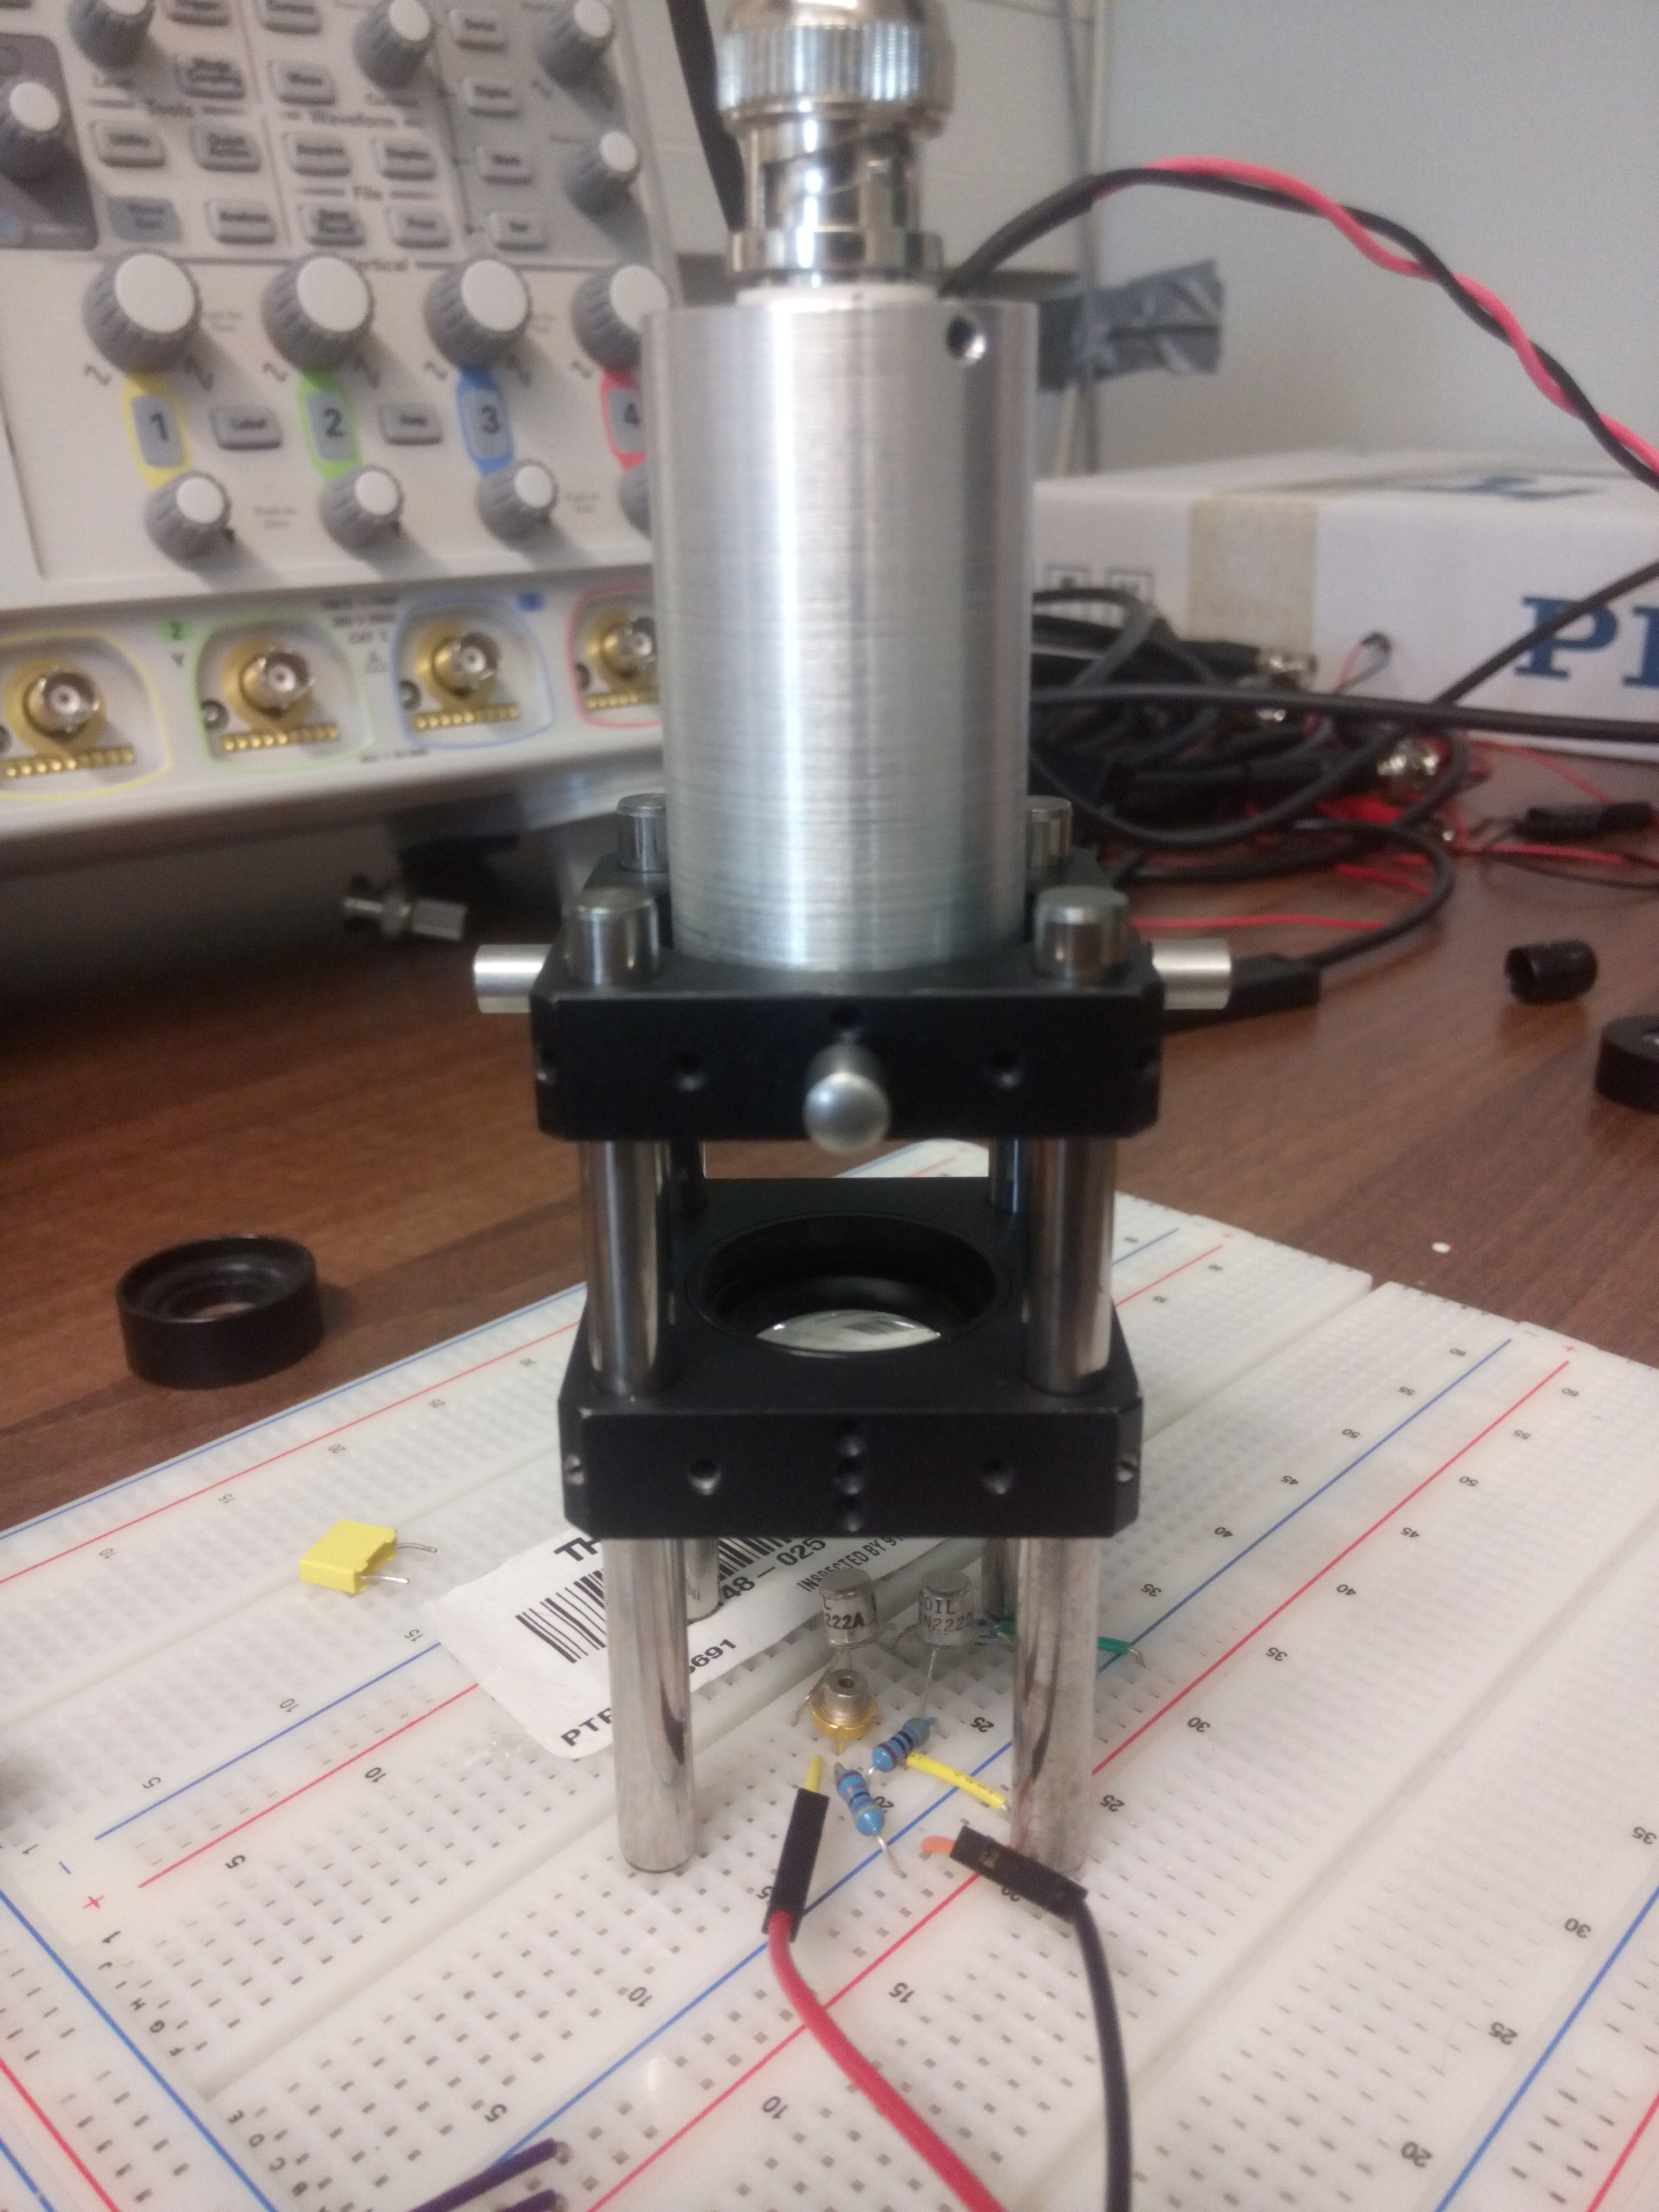
\includegraphics[width=0.6\textwidth]{../photos/IMG_20140710_184030.jpg}
  \caption{Versuchsaufbau zur Erstellung der Augendiagramme}
  \label{fig:eye_setup}
\end{figure}

In unserem Fall wurden die Augendiagramme in Abbildung~\ref{fig:eye_plots_slow} und Abbildung~\ref{fig:eye_plots_fast} mit der Sendeschaltung aus Abschnitt~\ref{sec:direct_tx} und der Empfängerschaltung aus Abschnitt \ref{sec:direct_rx_tia} aufgenommen. Der Aufbau ist in Abbildung~\ref{fig:eye_setup} zu sehen.

\begin{figure}[H]
  \centering
  \begin{subfigure}[b]{0.6\textwidth}
    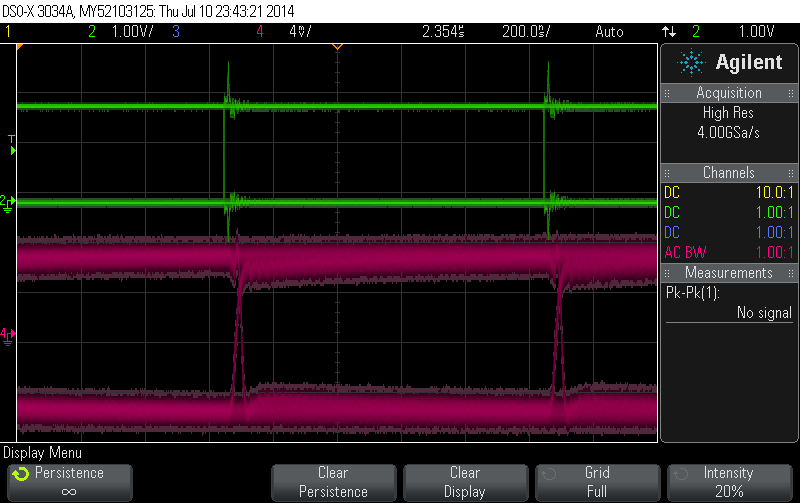
\includegraphics[width=\textwidth]{../measurements/20140710/eye_plots/01MHz.png}
    \caption{\SI{1}{\mega\hertz}}
    \label{fig:eye_plots_slow_1M}
  \end{subfigure}  
  \begin{subfigure}[b]{0.6\textwidth}
    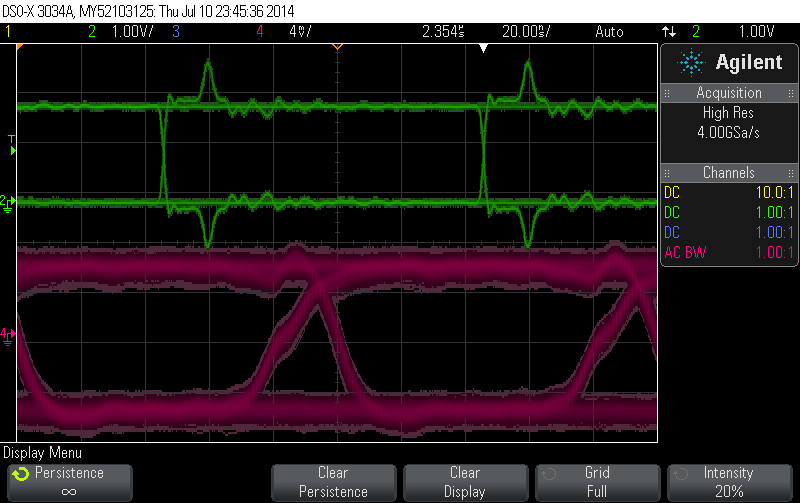
\includegraphics[width=\textwidth]{../measurements/20140710/eye_plots/10MHz.png}
    \caption{\SI{10}{\mega\hertz}}
    \label{fig:eye_plots_slow_10M}
  \end{subfigure}  
  \caption{Augendiagramme (gesendetes Signal in grün)}
  \label{fig:eye_plots_slow}
\end{figure}

\begin{figure}[H]
  \centering
  \begin{subfigure}[b]{0.6\textwidth}
    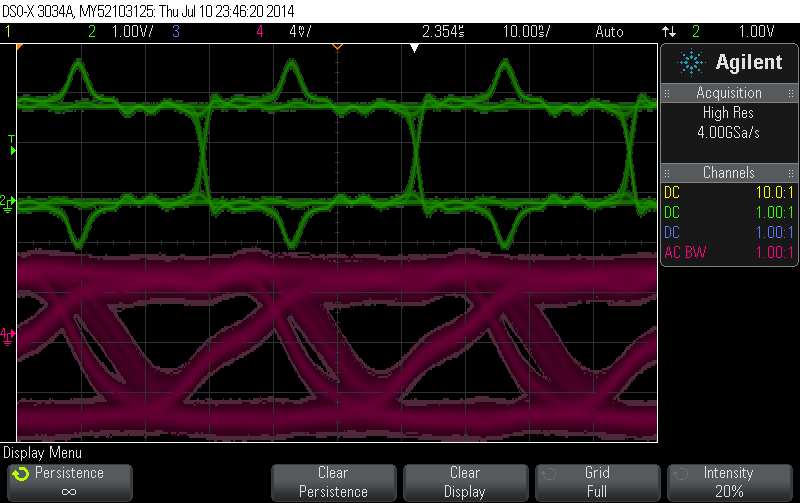
\includegraphics[width=\textwidth]{../measurements/20140710/eye_plots/30MHz.png}
    \caption{\SI{30}{\mega\hertz}}
    \label{fig:eye_plots_fast_30M}
  \end{subfigure}
  \begin{subfigure}[b]{0.6\textwidth}
    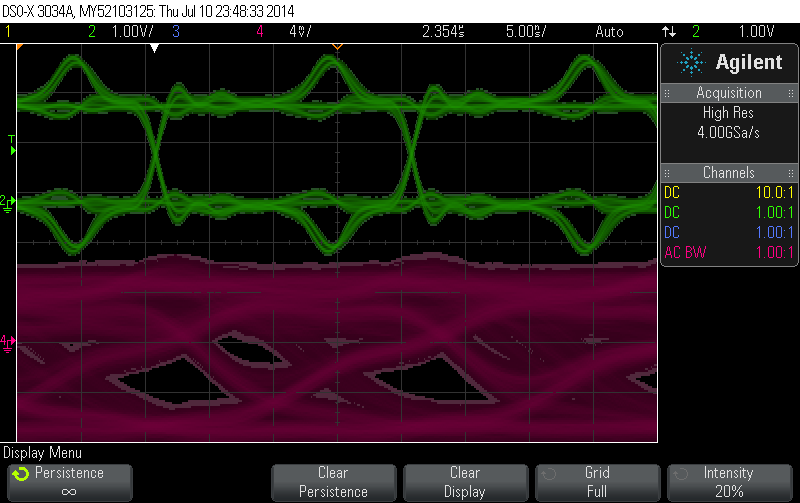
\includegraphics[width=\textwidth]{../measurements/20140710/eye_plots/50MHz.png}
    \caption{\SI{50}{\mega\hertz}}
    \label{fig:eye_plots_fast_50M}
  \end{subfigure}  
  \caption{Augendiagramme (gesendetes Signal in grün)}
  \label{fig:eye_plots_fast}
\end{figure}


Ein \SI{1}{\mega\hertz}-Bitsignal wird ohne Probleme übertragen (\ref{fig:eye_plots_slow_1M}), auch bei einem \SI{10}{\mega\hertz}-Signal ist die Augenöffnung noch unproblematisch (\ref{fig:eye_plots_slow_10M}). Ein \SI{30}{\mega\hertz}-Signal hat bereits eine deutlich kleinere Öffnung (\ref{fig:eye_plots_fast_30M}), die Übertragung sollte hier aber auch noch funktionieren. Bei \SI{50}{\mega\hertz} scheint die Grenze erreicht; hier ist eine distinkte Öffnung kaum noch zu erkennen (\ref{fig:eye_plots_fast_50M}). 

\subsection{Ergebnisse}
Mit dem System aus selbst gebauter modulierbarer Stromquelle und \textit{AD8015}-Verstärker lassen sich Signale mit einer Geschwindigkeit von bis zu \SI{50}{\mega\hertz} gut übertragen. Die Photodiode ohne Verstärker ist hingegen in diesem Geschwindigkeitsbereich nicht mehr zu gebrauchen.

Bezüglich des Senders sollte man als nächstes versuchen, die verwendete Schaltung wie in Abschnitt \ref{sec:direct_tx} beschrieben zu verbessern, um sie dann auf einer Platine aufzubauen. Zusammen mit einem Gehäuse ließe sich damit ein Versuchsaufbau erstellen, mit dem die Schaltung noch besser untersucht und der Laser auch in eine Glasfaser eingekoppelt werden könnte.

Der Empfänger mit \textit{AD8015} hat sich bewährt und muss wohl erst einmal nicht verändert werden. Es wäre aber interessant, ihn noch besser zu vermessen. Unter anderem sollte mit einer professionellen Lichtquelle untersucht werden, bis zu welchen Frequenzen verstärkt werden kann. Bisher wurde hier nur das Gesamtsystem aus Empfänger und Sender untersucht, was es erschwert, eindeutige Aussagen über die Einzelkomponente zu treffen. Interessant könnte es auch sein, die \textit{AD8015}-Schaltung mit verschiedenen Photodioden aufzubauen und zu untersuchen, wie sich diese auf das Verstärkungsverhalten auswirken.

\section{Fazit}

Auch wenn wir, insbesondere mit dem LCD, keine besonders großen Erfolge erzielen konnten, so war das Praktikum für uns dennoch sehr interessant und lehrreich. Es wurde klar, dass die Beschreibung als LTI-System nur eine Näherung ist, die sich nicht ohne Weiteres auf das LCD übertragen lässt. Es ist daher wichtig, mit Zufallsbitfolgen zu messen, um ein Einschwingen zu verhindern. Auch bedeutet ein einzelner Sinuston, der sich in guter Qualität übertragen lässt, noch lange nicht, dass man dynamische Musiksignale, die Frequenzen aus dem gesamten hörbaren Spektrum enthalten, übertragen kann.
\\\\
Im Nachhinein fallen einem zahlreiche Dinge ein, die man hätte besser machen können. So sei Studenten, die in Zukunft dieses Praktikum durchführen, empfohlen, von Anfang an strukturiert vorzugehen. So sollte man sich erst überlegen, welche Kenndaten des LCDs benötigt werden, und anschließend, wie diese zu messen sind. Sehr wichtig ist außerdem, immer daran zu denken, den Versuchsaufbau zu einer Messung genau zu dokumentieren, um Wiederholbarkeit sicherzustellen. So haben wir es leider versäumt, den genauen Aufbau bei Aufnahme der ersten Messungen mit dem LCD festzuhalten.

Darüber hinaus wäre interessant gewesen, einige Messreihen mit unterschiedlichen Arten der Ansteuerung des LCDs aufzunehmen. Hier wären Latenz (also Gruppenlaufzeit) und Amplitudenübertragungsfunktion interessant. Unter anderem könnte man den LCD mit verschiedenen Amplituden sowie mit oder ohne hochfrequenter Trägerwelle ansteuern.

Interessant war auch der praktische Einsatz von Kenntnissen aus \textit{Grundgebiete der Informatik \rom{2}} bei der Übertragung von Daten mittels eines Hamming-Codes. Hier zeigte sich, dass eine niedrigere Übertragungsgeschwindigkeit effizienter sein kann, da weniger Fehler erzeugt und somit weniger Paritätsbits benötigt werden. Für die Übertragung von digitalen Daten wäre es bei einer erneuten Durchführung des Praktikums interessant, nach Charakterisierung des LCDs eine Übertragungsstrecke mit niedrigerer Latenz zu konstruieren.

Bei der direkten Modulation des Lasers empfiehlt es sich, die Schaltung des Senders wie oben beschrieben zu optimieren und dann fest aufzubauen, um Messungen einfacher und genauer durchführen zu können. Beim Empfänger mit \textit{AD8015}-Verstärker könnte man Messungen mit einer modulierten Lichtquelle, deren Bandbreite bekannt ist, durchführen, um seine maximale Bandbreite zu ermitteln.
\\\\
Gelohnt hat sich definitiv auch, in der Exkursionswoche für zwei ganze Tage am Projekt zu arbeiten. So kann man einmal etwas mehr am Stück erledigen, ohne sich Woche für Woche erneut in das Projekt hineindenken zu müssen. Wir raten aber davon ab, dass Praktikum komplett an einem Stück durchzuführen, da dann nicht genug Zeit bleibt, um Teile zu bestellen oder Platinen fertigen zu lassen.
\\\\
Zu guter Letzt möchten wir den zukünftigen Teilnehmern dieses Praktikums viel Erfolg wünschen. Ihr könnt euch auf jeden Fall auf die Unterstützung des Instituts verlassen. Egal ob ihr Fragen habt, Hilfe oder Teile für die Durchführung braucht, wendet euch einfach an euren Betreuer.

Wir hoffen, dass wir euch mit unserem Projektbericht helfen konnten und würden uns freuen, in einem Jahr eure Ergebnisse zu sehen.
\\\\
Viel Spaß!

\appendix
\section{C++-Quellcode-Ausschnitte}
\label{app:code}

\subsection{Hamming-Code}
\label{app:code_hamming}
\inputminted[label=hamming.hpp,linenos,tabsize=4,fontsize=\normalsize,frame=lines,rulecolor=\color{gray!70},framerule=1pt]{c++}{../stm32/lcd_transmitter/hamming.hpp}
\url{https://github.com/ekiwi/iph/blob/master/stm32/lcd\_transmitter/hamming.hpp}

\subsection{Software-UART: Quelle}
\inputminted[label=transmitter.cpp,linenos,tabsize=4,fontsize=\normalsize,frame=lines,rulecolor=\color{gray!70},framerule=1pt]{c++}{../stm32/lcd_transmitter/source/transmitter.cpp}
\url{https://github.com/ekiwi/iph/blob/master/stm32/lcd\_transmitter/source/transmitter.cpp}

\subsection{Software-UART: Empfänger}
\label{app:uart_receiver}
\inputminted[label=receiver.cpp,linenos,tabsize=4,fontsize=\normalsize,frame=lines,rulecolor=\color{gray!70},framerule=1pt]{c++}{../stm32/lcd_transmitter/sink/receiver.cpp}
\url{https://github.com/ekiwi/iph/blob/master/stm32/lcd\_transmitter/sink/receiver.cpp}

\end{document}
